% Use only LaTeX2e, calling the article.cls class and 12-point type.

\documentclass[11pt]{article}

\usepackage[round,semicolon]{natbib}
\usepackage{etoolbox}
\AtBeginEnvironment{quote}{\singlespacing\tiny}
% Use times if you have the font installed; otherwise, comment out the
% following line.

% added by SKH
%\usepackage{lineno}
%\linenumbers

\usepackage{times}
\usepackage{amssymb}
\usepackage{amsmath}

\usepackage[export]{adjustbox}

\usepackage{graphicx}
\graphicspath{ {images/} }

% for adjustwidth
\usepackage{changepage}

% The following parameters seem to provide a reasonable page setup.

\topmargin 0.0cm
\oddsidemargin 0.2cm
\textwidth 16cm 
\textheight 21cm
\footskip 1.0cm

\usepackage{newfloat}
\usepackage{amsmath}
\usepackage[labelfont=bf]{caption}
\usepackage{nameref}
\usepackage{rotating}
\usepackage{color}
\usepackage{float}
\renewcommand{\figurename}{{}}
\renewcommand{\thefigure}{{Figure \arabic{figure}}}

\renewcommand{\tablename}{{}}
\renewcommand{\thetable}{{Table \arabic{table}}}

\newfloat{suppfile}{thp}{losuppfile}
\renewcommand{\thesuppfile}{Supplementary file \arabic{suppfile}}
\floatname{suppfile}{}

\newfloat{suppfig}{thp}{losuppfig}
\renewcommand{\thesuppfig}{Supplementary figure \arabic{suppfig}}
\floatname{suppfig}{}

%
\newfloat{supptable}{thp}{losupptable}
\renewcommand{\thesupptable}{Supplementary table \arabic{supptable}}
\floatname{supptable}{}
%

\renewcommand{\theequation}{Equation \arabic{equation}}

\newcommand{\mutDNA}{\textbf{mutDNA}}
\newcommand{\mutvirus}{\textbf{mutvirus}}
\newcommand{\DNA}{\textbf{DNA}}
\newcommand{\virus}{\textbf{virus}}

\newcommand\skhcomment[1]{{\color{cyan}[#1]}}
\newcommand\jdbcomment[1]{{\color{red}[#1]}}


\usepackage{hyperref}
\hypersetup{colorlinks,citecolor=blue,linkcolor=blue,urlcolor=blue}
\hypersetup{colorlinks,citecolor=blue,linkcolor=blue,urlcolor=blue}

\usepackage{seqsplit}

\usepackage{array}
\newcolumntype{P}[1]{>{\raggedright\arraybackslash}p{#1}}

\title{Experimentally informed site-specific substitution models deepen phylogenetic estimates of the divergence of viral lineages} 

\author
{Sarah K. Hilton$^{1,2}$  and Jesse D. Bloom$^{1,2}$\\
\\
\normalsize{$^1$Division of Basic Sciences and Computational Biology Program,}\\
\normalsize{Fred Hutchinson Cancer Research Center, Seattle, WA 98109, USA}\\
\normalsize{$^2$Department of Genome Sciences, University of Washington, Seattle, WA}\\
\normalsize{E-mail:  jbloom@fredhutch.org.}\\
}


% Include the date command, but leave its argument blank.

\date{}

\usepackage{setspace}
\onehalfspacing


\begin{document} 

% Make the title.

\maketitle 


\begin{abstract}
\noindent \skhcomment{$\leq$ 250 words, currently 217}   
Molecular phylogenetics is often used to estimate the time since the divergence of modern gene sequences.
Such phylogenetic techniques often estimate substantially shallower divergence times than other methods.
For instance, in the case of viruses there is independent evidence that molecular phylogenetics can underestimate deep divergence times.  
This discrepancy is thought to be caused in part by inadequate models of purifying selection leading to branch-length underestimation.
Here we show that substitution models informed by experimental measurements of site-specific purifying selection lengthen the branches on phylogenies of influenza virus hemagglutinin.
This deepening of branch lengths is due to better modeling how site-specific amino-acid preferences affect the stationary state of the substitution models, and is independent of the branch-length-extension due to modeling site-to-site variation in substitution rate.
We show that the deepening of branch lengths from experimentally informed site-specific substitution models is similar to that achieved by other approaches that allow the stationary state to vary across sites.
However, the improvements from these site-specific models are limited by the inherent tension between the enhanced accuracy of accounting for site-specific amino-acid preferences and the fact that these preferences shift over long evolutionary times.
Overall, our work underscores the importance of modeling how site-specific purifying selection affects the stationary state as well as the substitution rate when estimating deep divergence times. 
\end{abstract}

\clearpage

\section*{Introduction} 
\skhcomment{from JDB: what is the "age" of a virus? Maybe "divergence time of viral lineages"}
skhcomment{from JDB: what is the less than a million actually? "Old" is not the right phrase.}
Estimating the divergence time of viral lineages of a virus is essential to understanding its evolutionary history, including its emergence, spread, and past zoonoses. 
This estimation is commonly done using the concept a ``molecular clock" to transform the branch lengths of the viral phylogenetic tree into age in years. 
However, this molecular dating technique often underestimates the age of many viruses, including measles, foamy virus, and ebola \skhcomment{(citations)}, compared to other methods which are independent of the viral phylogeny. 
For example, SIV (the original source of HIV) is estimated to be less than a million years old based on the viral phylogeny \citep{sharp2000origins,wertheim2009dating,worobey2010island} but estimated to be several million years old based on the host tree or endogenous retroviral elements  \citep{compton2013host} \skhcomment{(other citations)}. 
Overall, there is a systematic and substantially large underestimation of of branch length on viral phylogenies. 
\skhcomment{long branches}

Branch length underestimation is due, in part, to strong purifying selection masking the evolutionary signal in the observed sequences. 
Purifying selection can lead to mutational saturation, where multiple unobserved, substitutions occur at a single site along a long branch and erase the divergence signal \citep{holmes2003molecular}.
Furthermore, proteins do not have equal preference for all amino acids at all sites, this evident by a simple visual inspection of a multiple sequence alignment. 
How many and which amino acids tolerated at each site of the protein generate a site-specific expected rate of change. 
Failing to account for these site-specific constraints will lead to branch length underestimation. 
\skhcomment{you will have mutational saturation no matter what - this is a separate, addressable issue?}
\skhcomment{talk about the high mutation rate in viruses?}

Substitution models that incorporate site-to-site rate variation have been developed to decrease the bias in long branch estimation. 
The most common strategy is to allow a single rate-controlling parameter to vary according to some statistical distribution, such as a $\Gamma$-distributed $\omega$ (~dN/dS) \citep{yang2000codon}. 
This flexibility in the value of $\omega$ accounts for the site-to-site rate variation by allow some sites to have a higher dN/dS value than others. 
While this modification is simple and only requires the addition of one extra parameter, it does not describe site-specificity in its stationary state. 
That is, at evolutionary equilibrium, this model still assumes that each site in the protein evolves identically.  

An alternative approach is to model the site-specific amino-acid frequencies explicitly, such as those models in the mutation-selection family \citep{halpern1998evolutionary}. 
In these models, each amino-acid at each site in the protein is described by its own parameter and these differences are reflected in the stationary state of the model. 
The rate of change at a given site is controlled by these amino acid profiles and can now vary from site to site, as expected based on observations in nature. 
Importantly, these rate variations are not constrained to an arbitrary statistical distribution but by parameters with a direct biological interpretation. 

Mutation-selection models are presumably more biologically relevant but pose more practical challenges than the $\Gamma\omega$ models. 
These models are highly parametrized with 19 free parameters (the 20 amino acid preferences are constrained to sum to one) per site leading to thousands of parameters for the length of a normal protein. 
One way to avoid overfitting is to implement the model as a mixture model in either a bayesian \citep{lartillot2004bayesian} or maximum likelihood framework \citep{si2008empirical}. 

Alternatively, you can reduce the parameter space by defining the amino-acid frequencies \textit{a priori}. 
We have shown previously that we can define an Experimentally Informed Codon Model (ExpCM) \citep{bloom2014experimentally,bloom2014informed} from the mutation-selection family using measurements from deep mutational scanning \citep{fowler2014deep}, a high-throughput functional assay. 
ExpCM are therefore defined by amino-acid preferences measured in a \textit{single} genetic background and do not reflect any epistatic changes which may have occurred over the virus's evolutionary history. 
But they contain no more parameters than the traditional codon models while maintaining a site-specific stationary state. 
We hypothesize that the ExpCM will estimate longer branches than the traditional models due to the protein-specific description of purifying selection. 
\skhcomment{CAT model has been shown to work well (better) on saturated data.}

In order to test this hypothesis, we compared the branch lengths of a influenza virus HA phylogenetic trees optimized by different substitution models. 
We found that the ExpCM did extend the length of branches from the focal sequence on the tree \skhcomment{define focal} and that this extension was seen even in the context of $\Gamma$-distributed rate variation. 
Furthermore, we found this extension occurred even in the presence of $\Gamma$-distributed $\omega$, indicating that they are both important for modeling purifying selection. 
This supports the conclusion that modeling purifying selection, especially in a model with a non-uniform stationary state, is important to estimating the branch lengths on phylogenetic trees. 

\section*{Results and Discussion}

\subsection*{Substitution models}

\begin{figure}[H]
\centerline{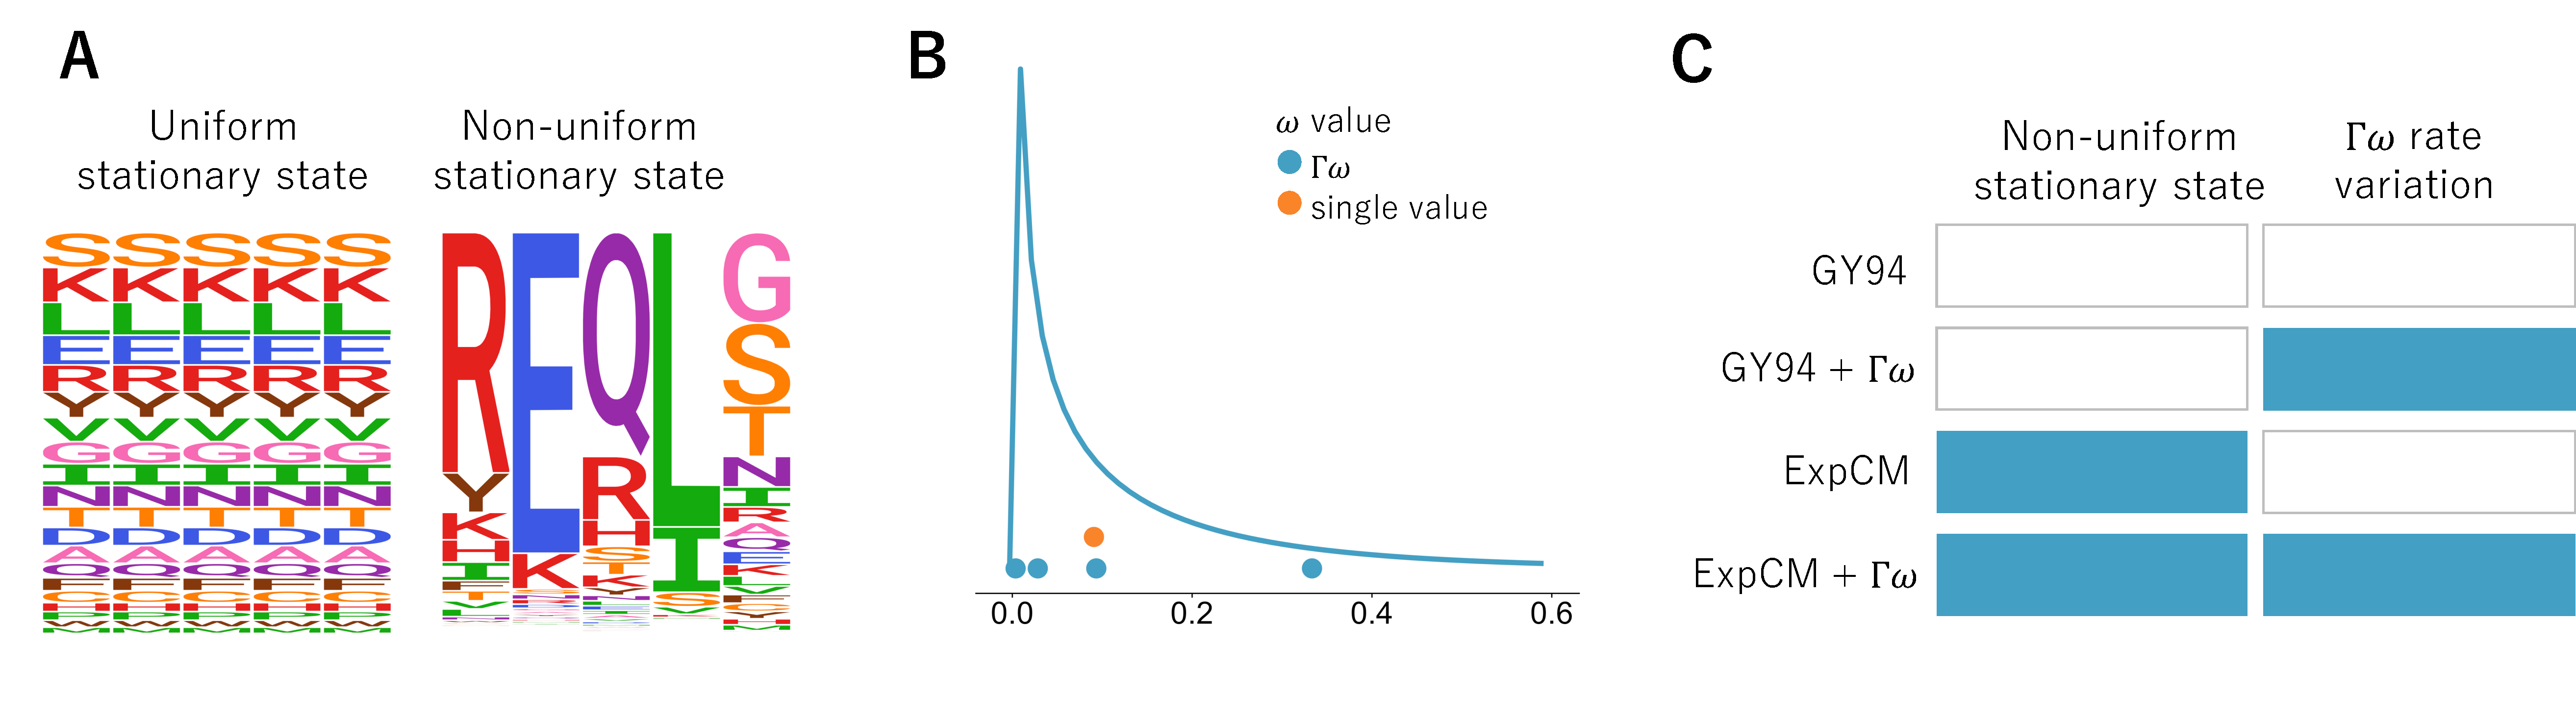
\includegraphics[width=0.90\textwidth]{figures/model_feature.pdf}}
\caption{\label{fig:model_feature}
\textbf{Comparison of substitution model features.}
(A) Substitution model stationary states can either be identical at every site in the protein or allow to vary from site to site. 
(B) The relative rate of non-synonymous change, $\omega$, can be defined as one, gene-wide average or allowed to vary following some statistical distribution. 
To ensure computational tractability, $\omega$ takes on the mean value of $K$ bins ($K=4$ shown). 
(C) Substitution models can both, one, or neither of these features. 
We used models from the GY94 and the ExpCM families. 
}
\end{figure}

It is well known that protein sites evolve under different pressures. 
Some sites appear to tolerate many amino acids while other sites appear to tolerate only a select few. 
Therefore, it is important to use substitution models which are able to describe this purifying selection, and the resulting site-to-site rate variation, when modeling protein evolution. 

The standard strategy to account for purifying selection is to allow the rate of non-synonymous change to vary among sites following some statistical distribution. 
This variation is commonly implemented by allowing the rate parameter, $\omega$, to follow a $\Gamma$-distribution ($\Gamma\omega$).
In order to achieve computational tractability, the distribution is discretized into $K$ bins and $\omega$ is assigned to the mean of each bin and the site likelihood is the average likelihood given each of the $\omega$ values. 
Under this model, some sites would have a higher rate of non-synonymous change than others but this rate would be agnostic to the amino-acid identities themselves. 
All non-synonymous changes would be treated as equally. 

Another strategy to account for purifying selection is to define a substitution model with a site-specific stationary state. 
Such models describe the evolution at each site uniquely and independently of the other sites. 
For example, models from the Halpern-Bruno mutation-selection family explicitly describe the frequency of each amino acid at each site. 
However, these more mechanistic models, without an arbitrary statistical distribution, come at a cost in the form of an increased number of parameters. 
When using a mutation-selection model is crucial to invoke a strategy to avoiding overfitting the data. 
We chose to define the amino-acid frequency parameters \textit{a priori} using measurements from a high-throughput functional assay called deep mutational scanning, Experimentally Informed Codon Models (ExpCMs).

These two strategies, $\Gamma\omega$ rate variation and non-uniform stationary states, are not truly distinct. 
Differences in stationary state manifest as differences in non-synonymous rates across sites \citep{spielman2015relationship}. 
Moreover, these two strategies are not mutually exclusive. 
Technically, substitution models can have a non-uniform stationary state and $\Gamma\omega$ rate variation and biologically, these models can account for both strong purifying and strong positive selection. 

\subsection*{Effect of stationary state and rate variation on branch length estimation}

\begin{figure}[H]
\centerline{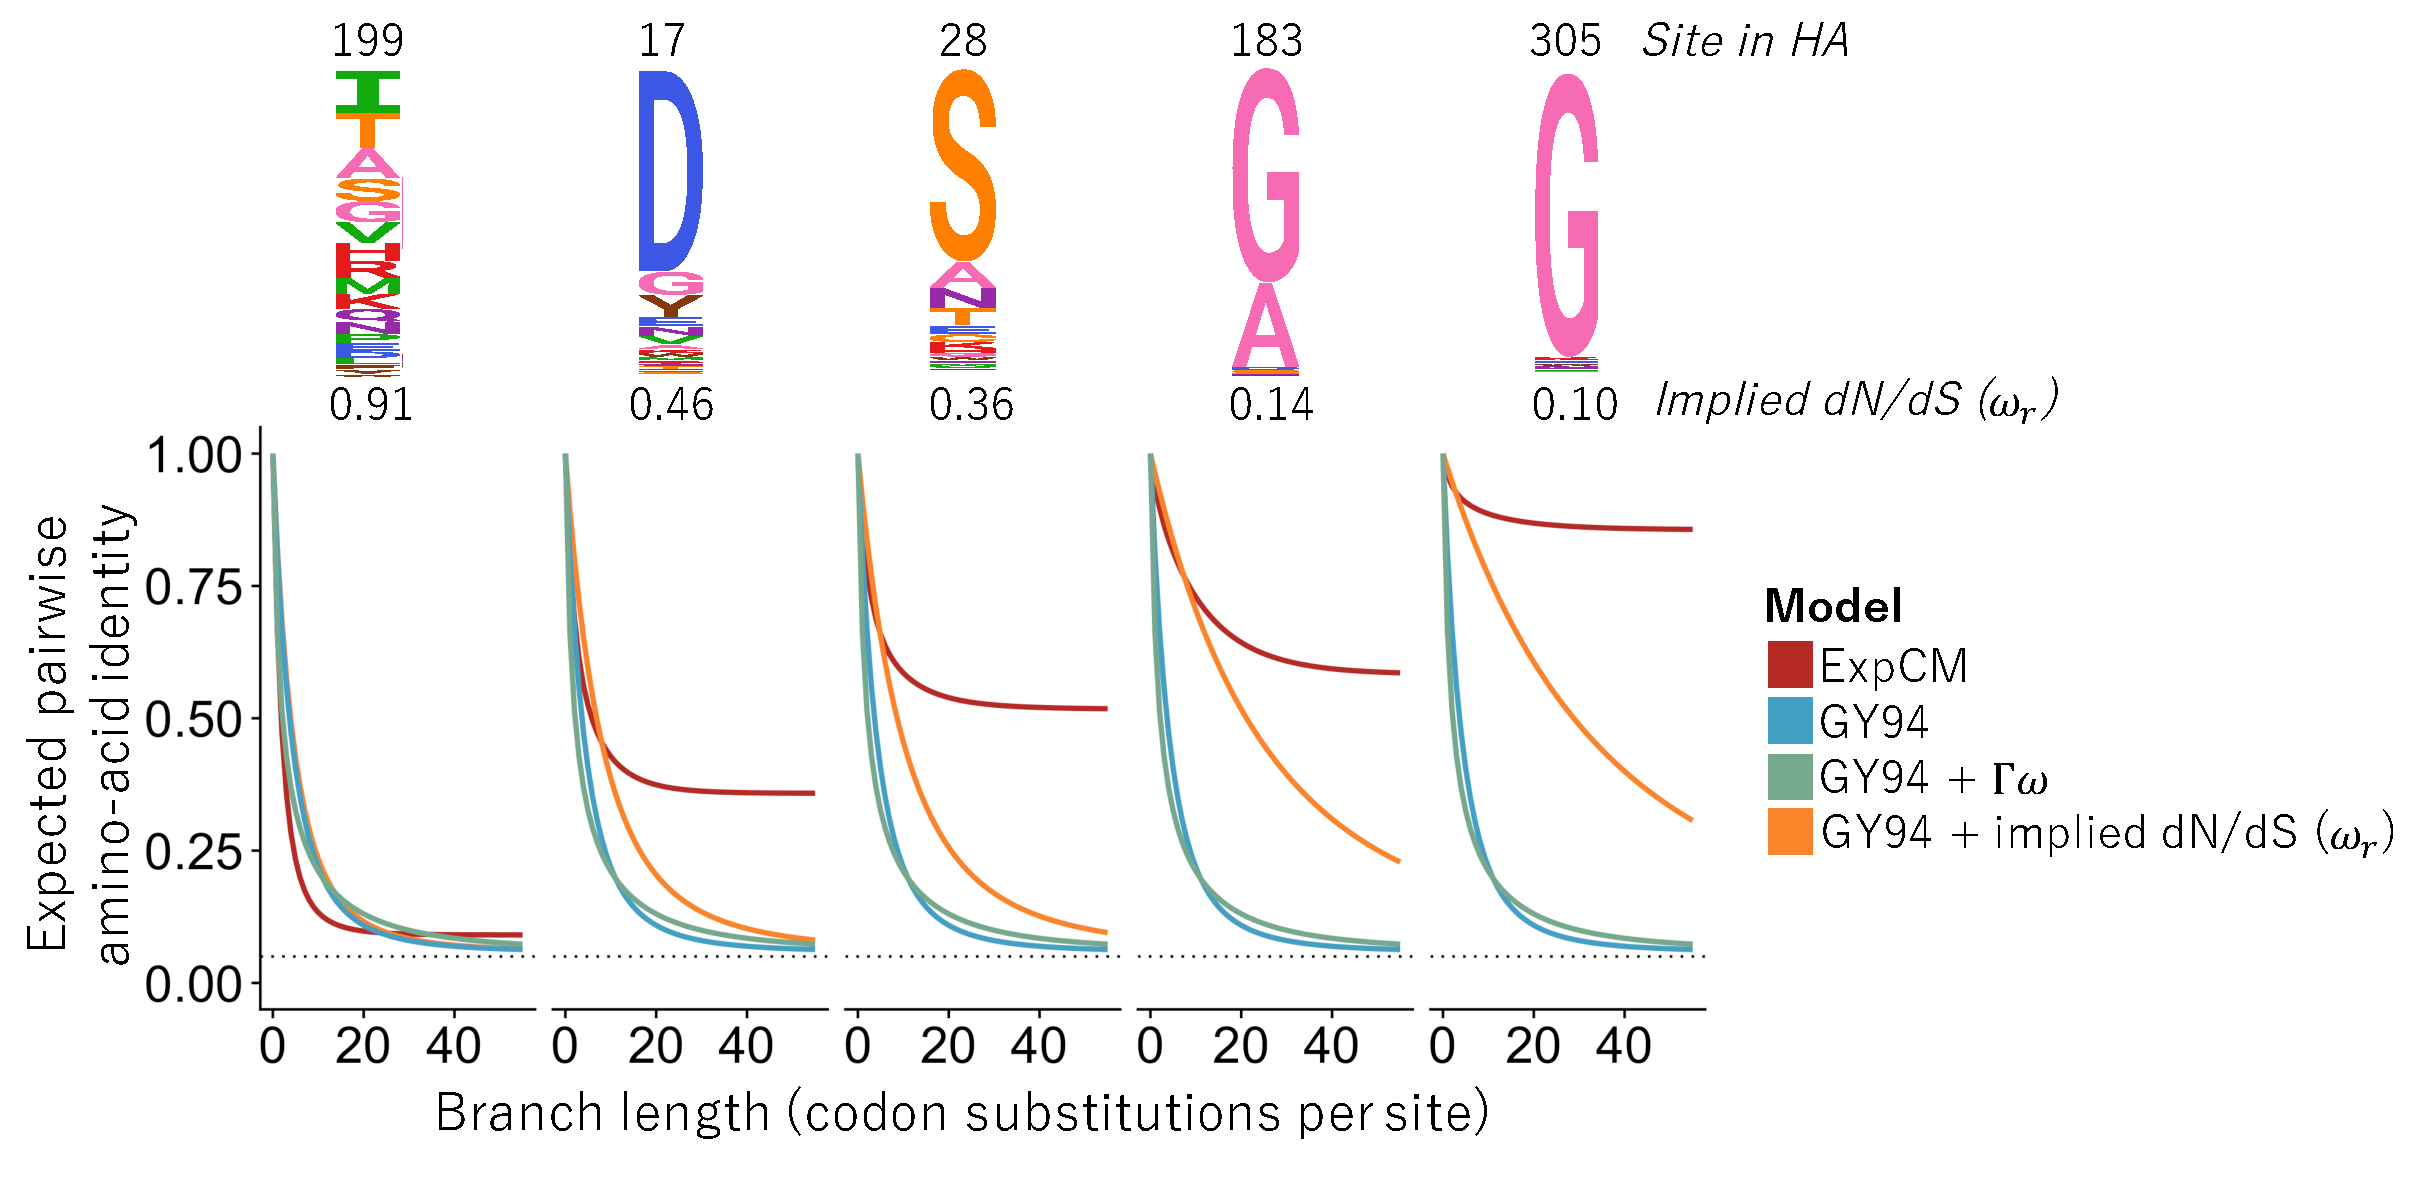
\includegraphics[width=0.90\textwidth]{figures/decay.pdf}}
\caption{\label{fig:decay}
\textbf{Effect of stationary state and rate variation on long branch estimation.}
The expected pairwise amino-acid identity for five sites in influenza hemagglutinin (HA) for four different substitution models. 
The logoplots show the HA amino-acid preferences from a deep mutational scan performed by \cite{doud2016accurate}. 
The implied dN/dS value was calculated from the ExpCM following \cite{spielman2015relationship}.
}
\end{figure}

Along a single branch, a substitution model transforms sequence divergence to branch length, which under a molecular clock assumption is proportional to time. 
However, every substitution model has a stationary state, the expected sequence divergence given a very long time, at which the relationship between sequence divergence and time is lost. 
The stationary state is represented by the long ``tails" in \ref{fig:decay}, where the expected sequence divergence remains constant as time increases. 

A substitution model's stationary state is defined by the parameters in the model and can vary from model to model. 
Some model features affect how long it takes a model to reach its stationary state, whereas other features affect the stationary state itself. 
Adding $\Gamma\omega$ rate variation affects the ``path" to the stationary state but does not affect the stationary state itself. 
In addition, while $\Gamma\omega$ accounts for site-to-site rate variation, the resulting stationary state is identical at each site in the protein. 
Under these models with uniform stationary states, a mutationally constrained site and a site which tolerates many mutations will have the sequence divergence given a very long time. 
Models with non-uniform stationary states, by definition, acknowledge that differences in sites will persist even at a very long period of time. 
The difference in branch length estimation will be most dramatic at constrained sites in the protein. 
At a constrained site, the ExpCM will estimate a longer branch than the GY94 model because the overall sequence divergence at that site is expected to be small.

This difference in branch length estimation cannot be recapitulated by more complex modeling of the $\omega$ parameter. 
We transformed the GY94 model into a site-specific model by inferring a unique $\omega$ value from the ExpCM, following the work of \cite{spielman2015relationship}, for each site in the protein. 
This model takes longer to reach stationary state than the GY94 model ultimately has the same divergence level at stationary state. 
As this model shows, no matter how ``well" a model accounts for site-to-site rate variation, it will underestimate long branches with a uniform stationary state model.  

\subsection*{Failure to account for site-specificity leads to branch length underestimation.}

\begin{figure}[H]
\centerline{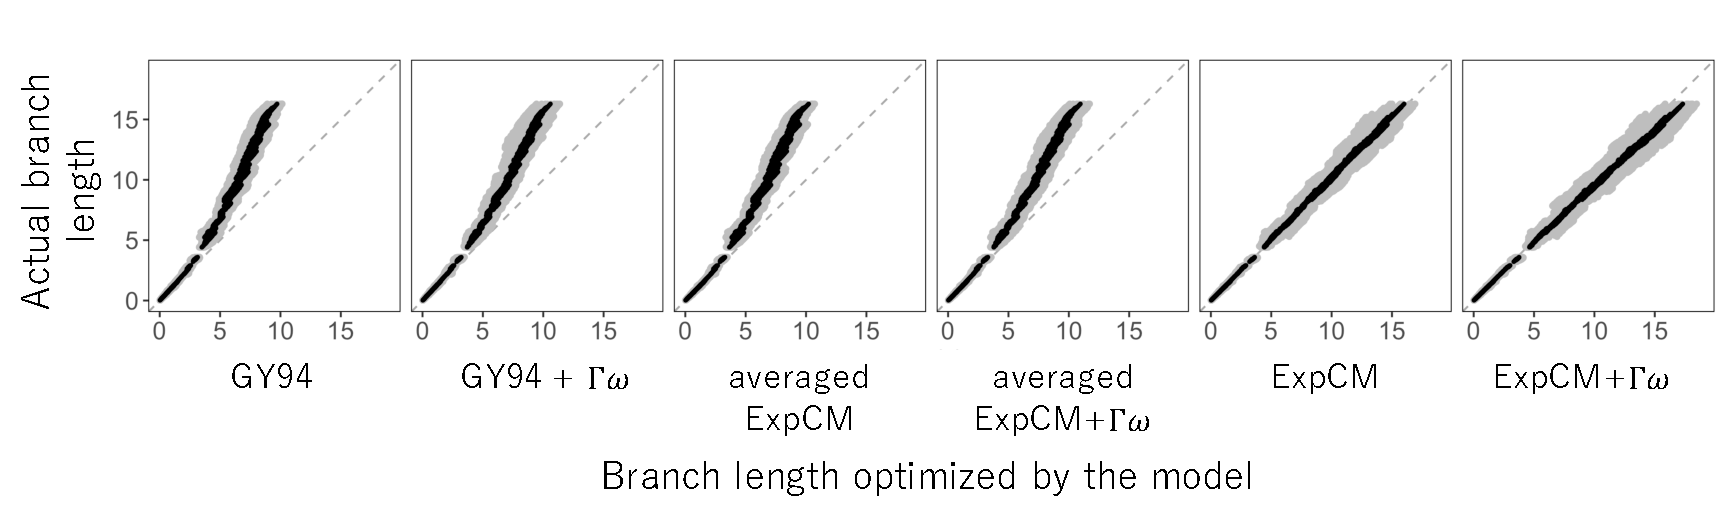
\includegraphics[width=0.85\textwidth]{figures/simulations}}
\caption{\label{simulations}
\textbf{Model performance under simulated, site-specific data.} 
Alignments were simulated under an ExpCM (\ref{tab:sim_params}) along an HA tree and the branches were re-optimized by a model from the ExpCM or YNGKP family. 
The randomized ExpCMs have amino-acid profiles shuffled among the sites 
These randomized models are still site-specific but the relationship between the site and the experimental data is broken. 
Grey points represent the length of one branch and the black points are the mean branch lengths over eight simulations. 
The grey, dashed line is the reference line $y=x$, depicting the behavior of a model which is an unbiased estimator of the simulated branch length. 
}
\end{figure}

First, we wanted to test the effect of substitution models on branch length estimation given sequences with site-specific amino-acid frequencies. 
To this end, we simulated sequences under and ExpCM and re-inferred the branch lengths using the different substitution models described in \ref{fig:model_feature}C. 
This allowed us to test whether or not a model with a uniform stationary state could accurately estimate branch lengths and, if not, whether or not the addition of $\Gamma\omega$ could prevent branch length underestimation. 

As expected, the ExpCM and ExpCM+$\Gamma\omega$ estimated the branch lengths of the simulated sequences accurately. 
As the branch lengths increase, the variance in the estimation of an given branch increases between the simulations but this error is not biased towards over- or underestimation.

The models with a uniform stationary state consistently underestimate the long branches. 
This underestimation is seen with both the GY94 and the GY94+$\Gamma\omega$, indicating that accounting for rate variation via the rate parameter cannot prevent branch length underestimation at these long branches. 
The ExpCM can also be transformed into a uniform stationary state model by setting the amino-acid at every site to the average value for that amino acid across all sites. 
In contrast to the GY94 models, this average control does not have preference for amino acid and does extract some information from the experiments, but like the GY94 models the stationary state is uniform across sites. 
These models performed similarly to the GY94 and GY94+$\Gamma\omega$ and underestimate long branches. 

These simulations show that when the sequences have site-specific amino-acid frequencies, models with uniform stationary states cannot accurately estimate branch lengths and, will in fact, underestimate long branches. 	

\subsection*{empirical Data}

\begin{figure}[H]
\centerline{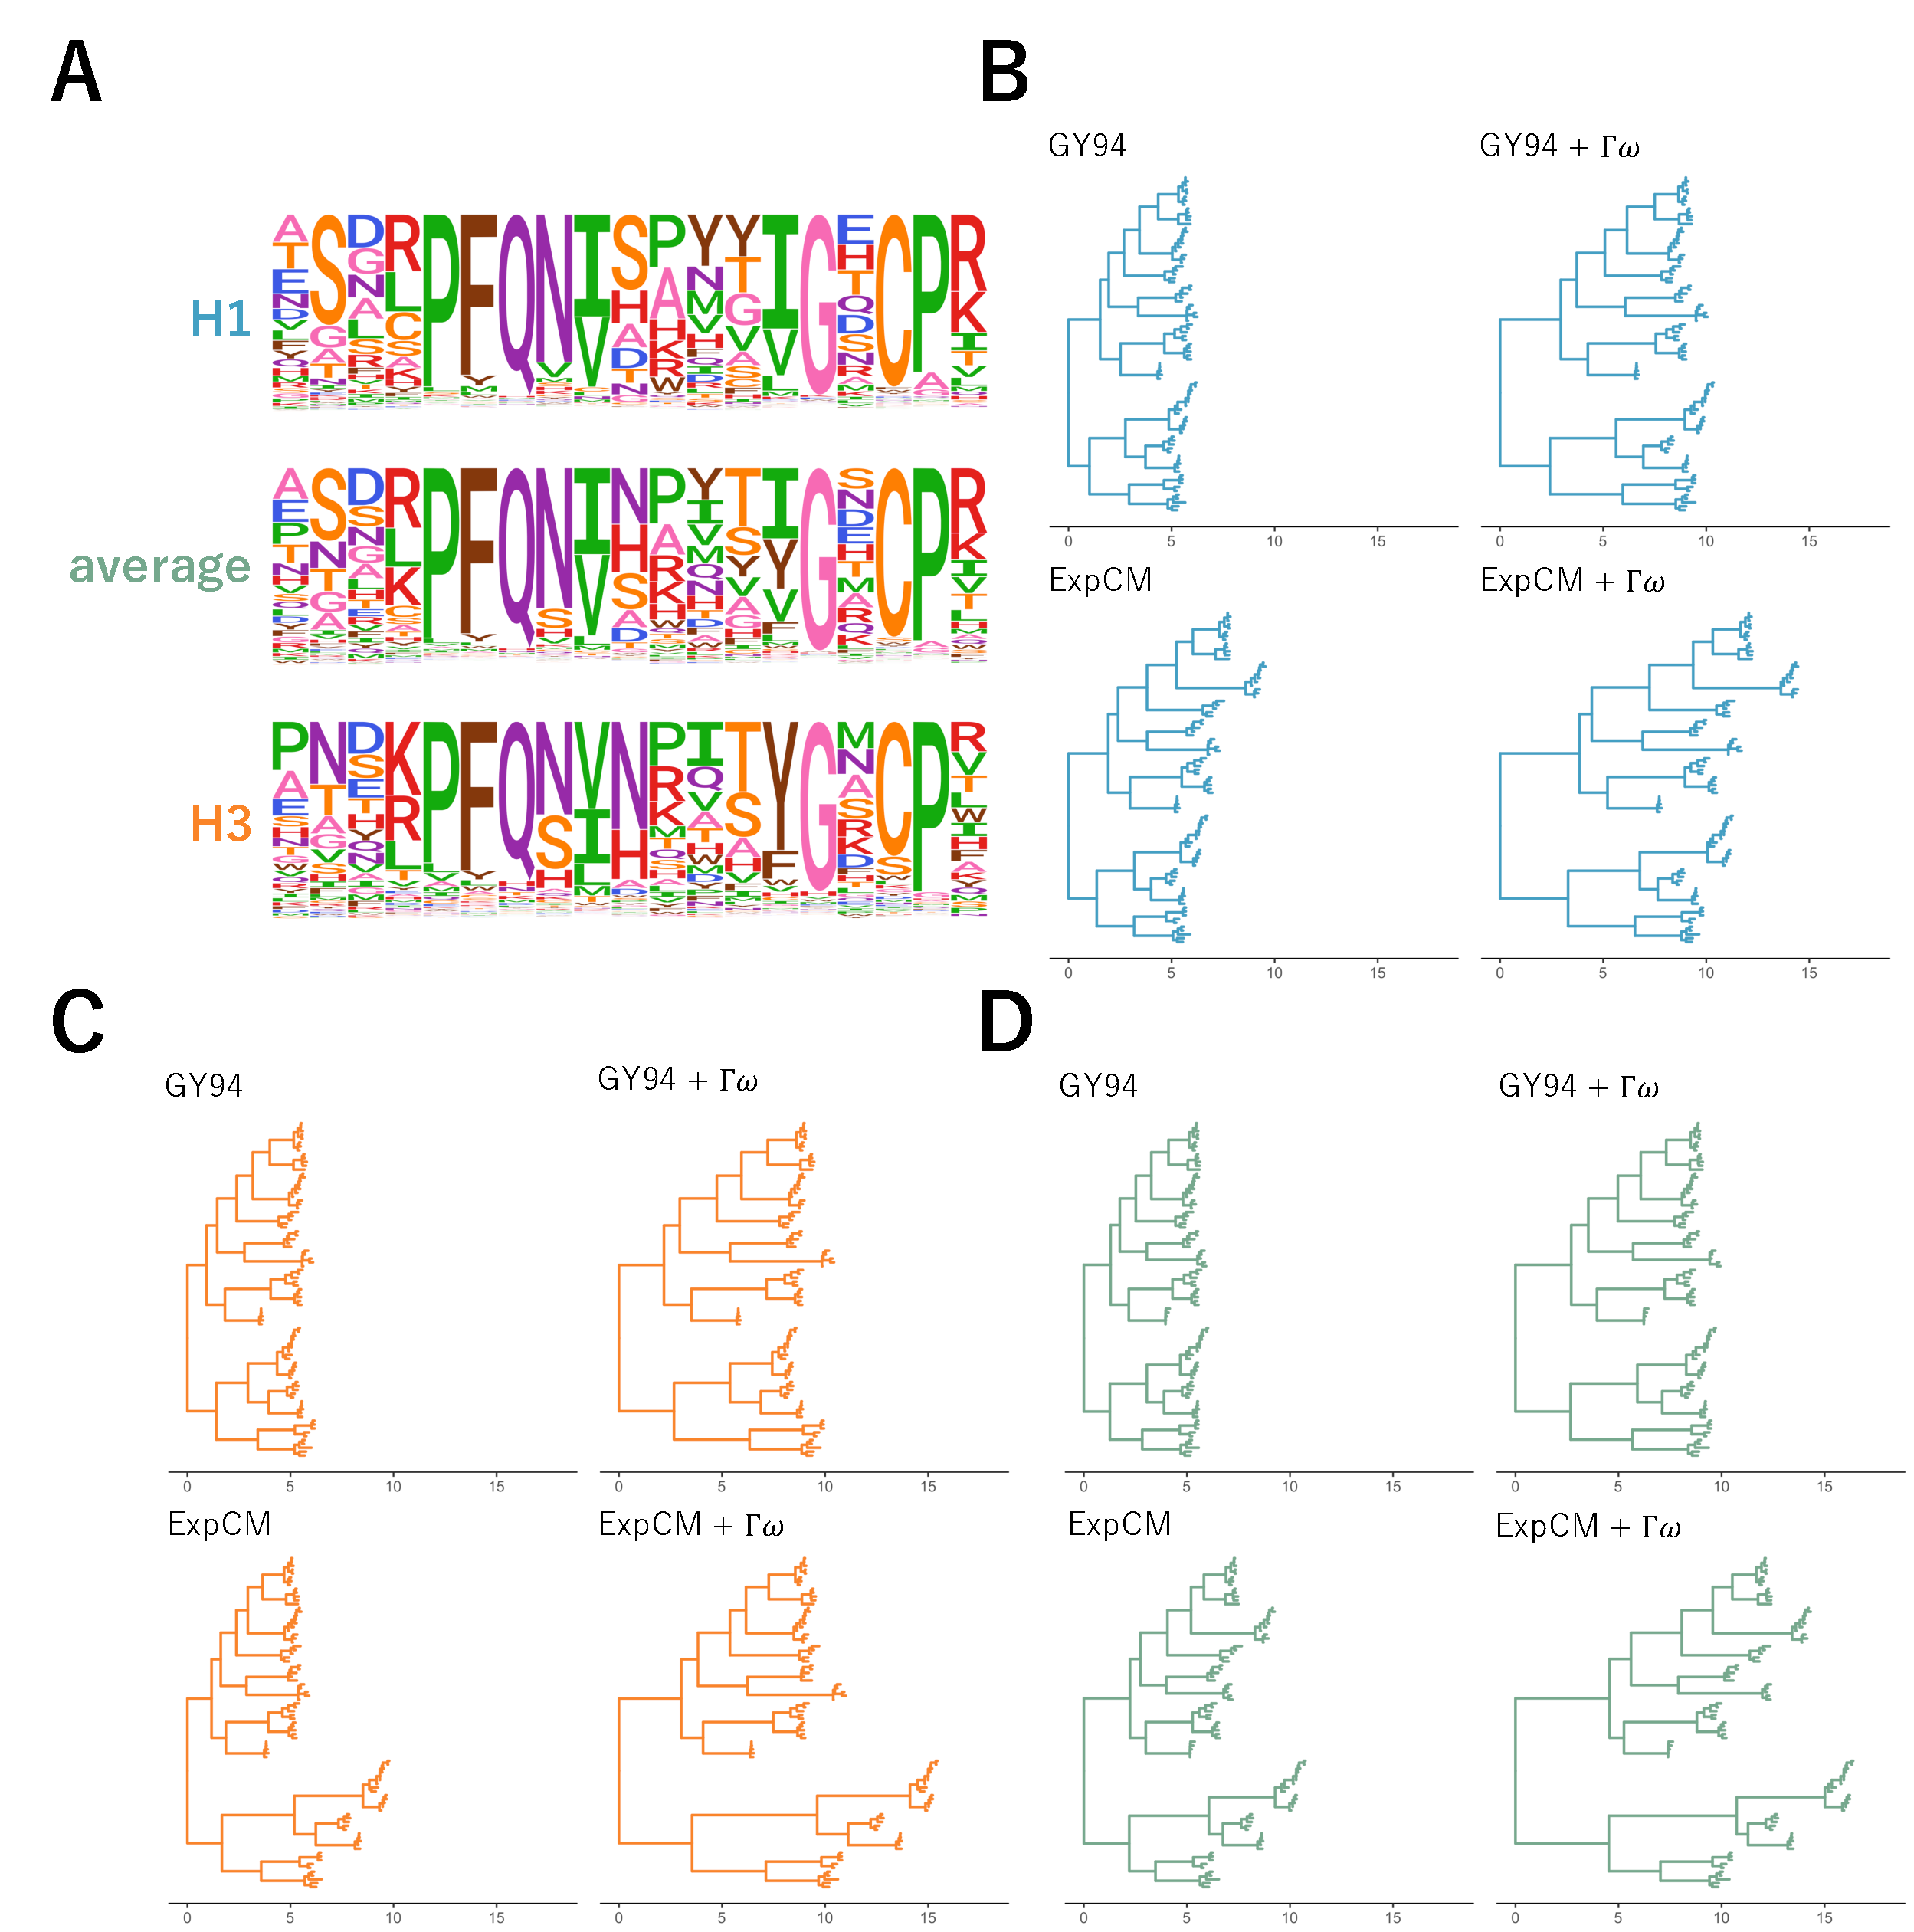
\includegraphics[width=0.9\textwidth]{figures/empirical_trees.pdf}}
\caption{\label{fig:empirical_trees}
\textbf{Trees optimized with an ExpCM defined by H1 preferences lengthen branches from the focal H1 sequence compared to YNGKP models.} 
\jdbcomment{Keep branch lengths in substitutions per site. Make a panel A show a prefs snippet, B H1 trees, C H3 trees, D H1+H3. Maybe increase very small font sizes a bit.}
The branch lengths of a base topology inferred using the GTR-CAT model were optimized by \textbf{(A)} an ExpCM defined by H1 preferences, \textbf{(B)} an ExpCM+$\Gamma\omega$ defined by H1 preferences, \textbf{(C)} YNKGP M0, and \textbf{(D)} YNGKP M5.
The branch lengths are normalized to the distance between A/South Carolina/1/1918 and A/Solomon Islands/3/2006 and colored to indicate the distance from the H1 focal sequence (black triangle).
}
\end{figure}

\begin{table}[t!]
\caption{\label{tab:empirical_data}
Model comparison for Fig.~\ref{fig:empirical_trees}.}
     \begin{tabular}{ccccc}
        \hline
          Model & $\Delta$AIC & Log Likelihood & Parameters\\ \hline
       	ExpCM + $\Gamma\omega$ (average) & 0.00 & -48751.16 & $\omega$ = (0.19,  0.50,  0.90,  1.86), $\beta=1.70$, $\kappa=3.73$\\
	ExpCM (average) & 949.70 & -49227.01 & $\beta=1.78$, $\kappa=3.40$, $\omega=0.15$\\
	ExpCM + $\Gamma\omega$ (H1) & 1306.44 & -49404.38  & $\omega$ = (0.13 ,  0.44,  0.91,  2.16), $\beta=1.12$, $\kappa=3.64$\\
	ExpCM + $\Gamma\omega$ (H3) & 1737.40 & -49619.86 & $\omega$ = (0.09,  0.33,  0.72,  1.77), $\beta=1.28$, $\kappa=3.71$\\
	ExpCM (H1) & 2555.58 & -50029.95 & $\beta=1.22$, $\kappa=3.24$, $\omega=0.13$\\
	ExpCM (H3) & 3196.50 & -50350.41 & $\beta=1.45$, $\kappa=3.38$, $\omega=0.12$\\
	GY94 + $\Gamma\omega$ & 4719.34 & -51105.83 & $\omega$ = (0.00,  0.03,  0.08,  0.26), $\kappa=3.18$\\
	GY94 & 7624.64 & -52559.48  & $\kappa=2.89$, $\omega=0.07$\\
      \end{tabular}
\end{table}

\skhcomment{Section Outline:}

\begin{itemize}
\item We tested the effect substitution model choice on branch length estimation using influenza HA sequences. 
\begin{itemize}
\item These sequences presumably evolve with site-specific frequencies but unlike the simulations we do not \textit{know} the model
\item These sequences are from fairly diverged proteins. Some sequences share only 40\% identity on the amino acid level 
\item The HA tree has closely related subtypes with long branches between subtypes.
\end{itemize}
\item Both $\Gamma\omega$ and non-uniform stationary states result in an extension of branch lengths. 
\begin{itemize}
\item The addition of $\Gamma\omega$ extends branches independent of preferences. 
\item The addition of preferences extends branches \textit{from the focal sequence} independent of $\Gamma\omega$. 
\end{itemize}
\item The extension of branch length from the focal sequence shows that the ExpCM does not have equal "relevance" across the whole tree. 
\begin{itemize}
\item This result is not entirely surprising. DMS measure the effects of single amino-acid changes in the context of a single genetic background. 
\item It is expected that there would be epistatic changes across such a highly diverged phylogenetic tree. ``Shifting preferences".
\end{itemize}
\end{itemize}

\subsection*{Competing effects of shifting preferences and long branches.}

\begin{figure}[H]
\centerline{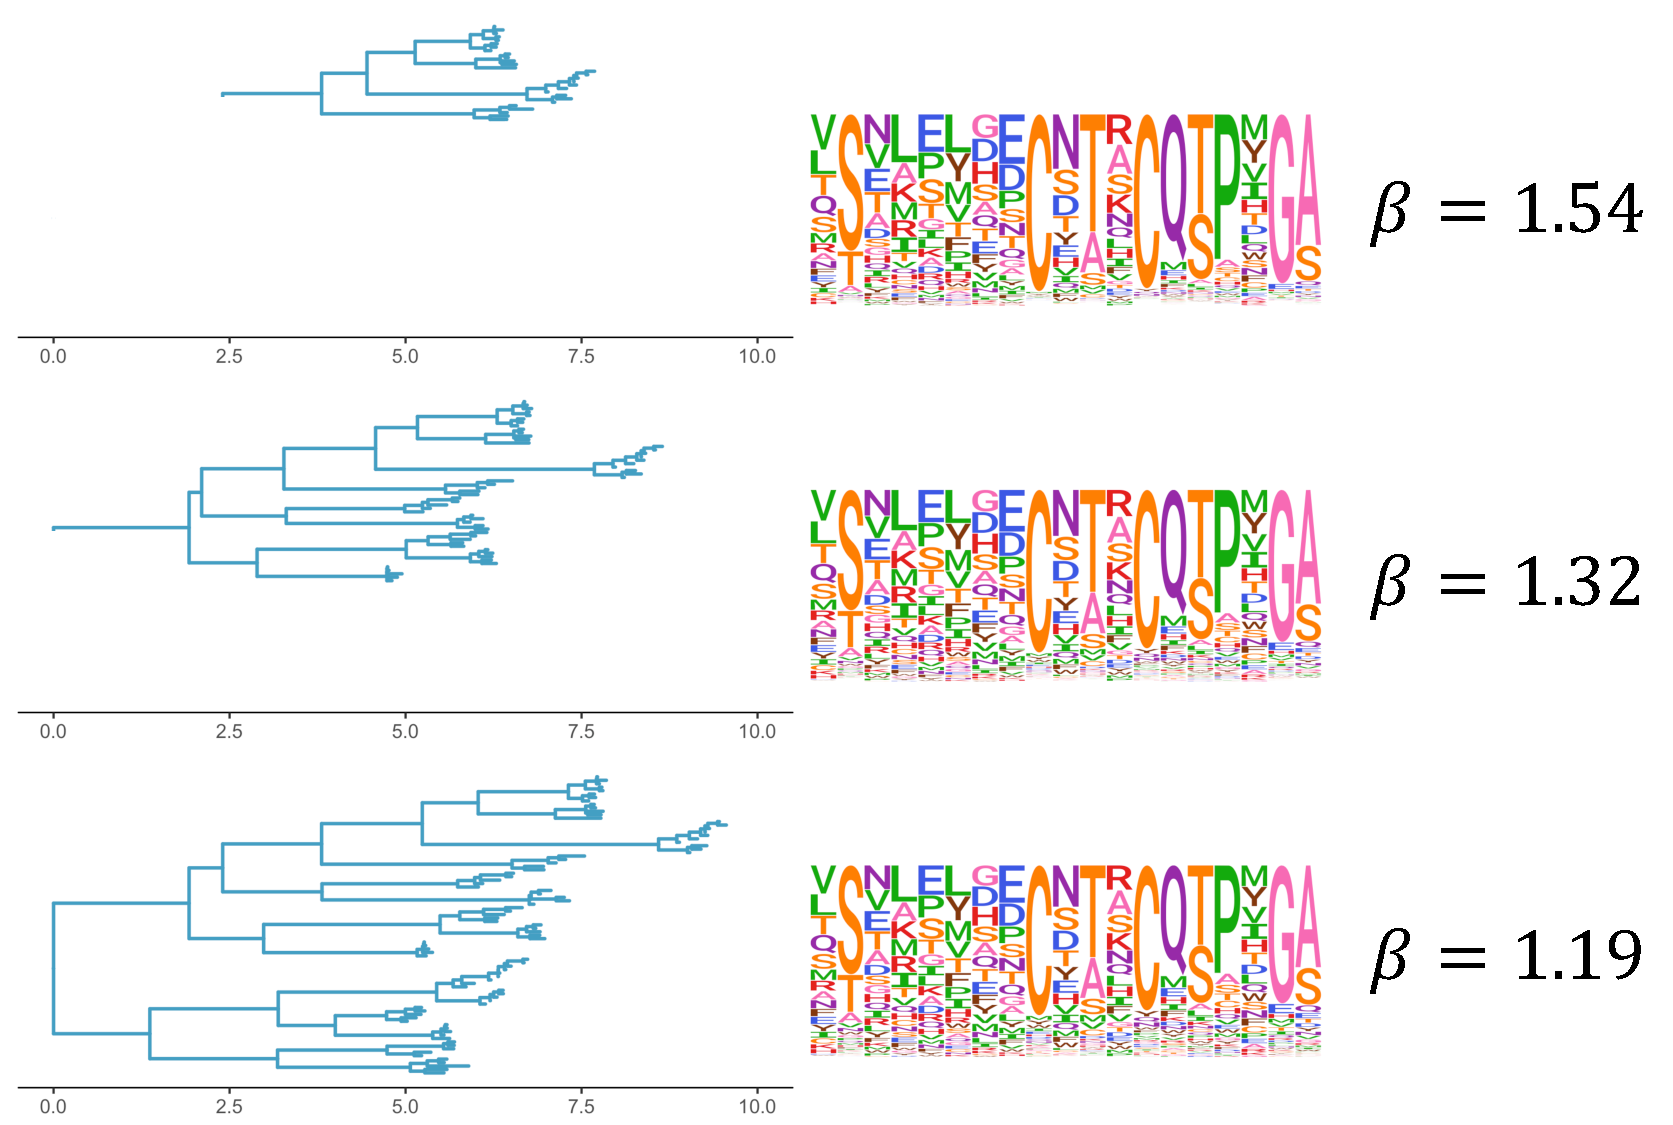
\includegraphics[width=0.85\textwidth]{figures/doud_compete_2}}
\caption{\label{fig:doud_compete}
\textbf{The ExpCM defined by H1 preferences lengthen longer branches on the HA tree.} 
\textbf{(A)} An HA alignment was subsampled to create three smaller alignments with varying degrees of divergence from the focal H3 sequence, referred to as "low", "intermediate", and "high". 
\textbf{(B)} The phylogenetic tree of the "high" alignment. 
The colors denote the alignment and the black circle denotes the focal H3 sequence. 
\textbf{(C)} The value of the ExpCM and ExpCM+$\Gamma\omega$ stringency parameter $\beta$ decreases as the divergence from the focal H3 sequence increases. 
\textbf{(D)} Comparisons of branch lengths optimized by the four substitution models for the varying degrees of divergence. 
Black points represent branches from the focal H3 sequence and grey points represent all other branches.  
The branch lengths are in average number of codon substitutions per site. 
}
\end{figure}

\skhcomment{Section Outline:}

\begin{itemize}
\item We investigated the competing effects of ``shifting preferences" and long branches by comparing ExpCMs with different "relevances"
\item We use the fit stringency parameter $\beta$ as a measure of relevance. 
\begin{itemize}
\item The stringency parameter rescales the preferences. A stringency parameter with a value greater than one indicates that selection in nature prefers the same amino acids as selection in lab but with greater strength. 
\item There is an inverse relationship between the stringency parameter and overall sequence divergence. As the overall divergence of the tree increases, the stringency parameter decreases. 
\end{itemize}
\item \skhcomment{hypothetical data} There is also a positive relationship between the stringency parameter and branch lengths 
\begin{itemize}
\item We optimized the same tree with ExpCMs with different stringency parameters. 
\item The ExpCMs with higher stringency values estimate longer branches than the ExpCMs with lower stringency values. 
\end{itemize}
\end{itemize}

\subsection*{\texttt{phylobayes}}

\begin{figure}[H]
\centerline{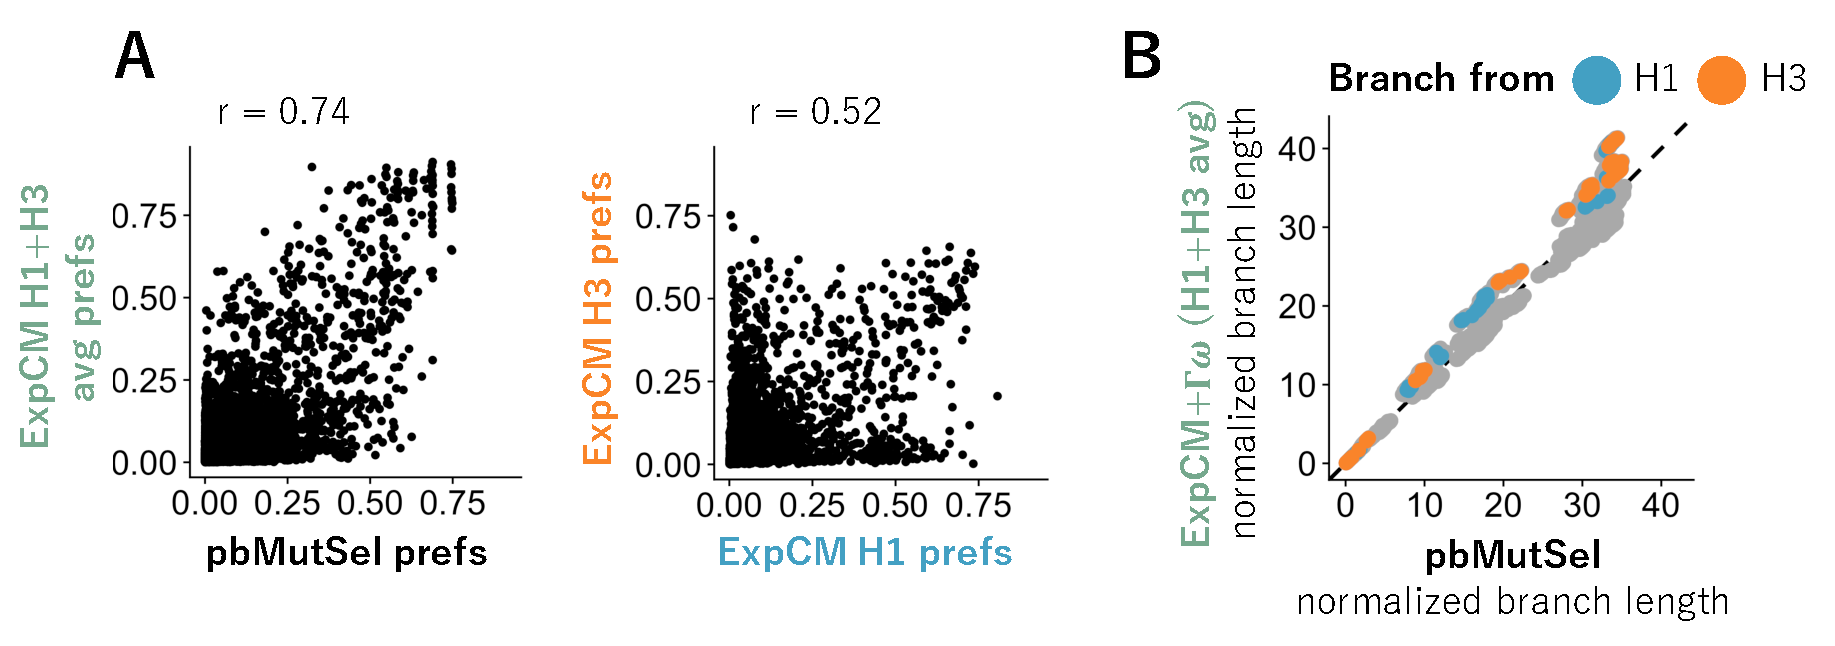
\includegraphics[width=0.5\textwidth]{figures/phylobayes.pdf}}
\caption{\label{fig:phylobayes}
\textbf{Comparison of ExpCM and phylobayes}
}
\end{figure}

\section*{Conclusion}

\begin{enumerate}
  \item We don't allow any of the models to vary by lineage. 
\end{enumerate}

\newpage
\section*{Materials and Methods}

\subsection*{Substitution models}
\subsubsection*{GY94 models}
\subsubsection*{ExpCMs}
We recap the \textbf{Exp}erimentally Informed \textbf{C}odon \textbf{M}odel (ExpCM) \citep{bloom2014experimentally,bloom2014informed,bloom2017identification,hilton2017phydms} to introduce nomenclature. 

In an ExpCM, rate of substitution $P_{r,xy}$ of site $r$ from codon $x$ to $y$ is written in mutation-selection form~\citep{halpern1998evolutionary,mccandlish2014modeling,spielman2015relationship} as
\begin{equation}
P_{r,xy} = Q_{xy} \times F_{r,xy}
\end{equation}
where $Q_{xy}$ is proportional to the rate of mutation from $x$ to $y$, and $F_{r,xy}$ is proportional to the probability that this mutation fixes.
The rate of mutation $Q_{xy}$ is assumed to be uniform across sites, and takes an HKY85-like~\citep{hasegawa1985dating} form:
\begin{equation}
Q_{xy} = 
\begin{cases}
\phi_w & \mbox{if $x$ and $y$ differ by a transversion to nucleotide $w$} \\
\kappa \phi_w & \mbox{if $x$ and $y$ differ by a transition to nucleotide $w$} \\
0 & \mbox{if $x$ and $y$ differ by $>1$ nucleotide.}
\end{cases}
\end{equation}
The $\kappa$ parameter represents the transition-transversion ratio, and the $\phi_w$ values give the expected frequency of nucleotide $w$ in the absence of selection on amino-acid substitutions, and are constrained by $1 = \sum_w \phi_w$.

The deep mutational scanning data are incorporated into the ExpCM via the $F_{r,xy}$ terms.
The experiments measure the preference $\pi_{r,a}$ of every site $r$ for every amino-acid $a$.
The $F_{r,xy}$ terms are defined in terms of these experimentally measured amino-acid preferences as
\begin{equation}
\label{eq:Frxy}
F_{r,xy} = 
\begin{cases}
   1 & \mbox{if $\mathcal{A}\left(x\right) = \mathcal{A}\left(y\right)$} \\
   \omega \times \frac{\ln\left[\left(\pi_{r,\mathcal{A}\left(y\right)} / \pi_{r,\mathcal{A}\left(x\right)}\right)^{\beta}\right]}{1 - \left(\pi_{r,\mathcal{A}\left(x\right)} / \pi_{r,\mathcal{A}\left(y\right)}\right)^{\beta}} & \mbox{if $\mathcal{A}\left(x\right) \ne \mathcal{A}\left(y\right)$}
   \end{cases}
\end{equation}
where $\mathcal{A}\left(x\right)$ is the amino-acid encoded by codon $x$, $\beta$ is the stringency parameter, and $\omega$ is the relative rate of nonsynonymous to synonymous substitutions after accounting for the amino-acid preferences.
The ExpCM has six free parameters (three $\phi_w$ values, $\kappa$, $\beta$, and $\omega$).
The preferences $\pi_{r,a}$ are \emph{not} free parameters since they are determined by an experiment independent of the sequence alignment being analyzed.

The ExpCM stationary state frequency $p_{r,x}$ of codon $x$ at site $r$ is~\citep{bloom2017identification} 
\begin{equation}
\label{eq:p_rx}
p_{r,x} = \frac{\left(\pi_{r,\mathcal{A}\left(x\right)}\right)^{\beta} \phi_{x_0} \phi_{x_1} \phi_{x_2}}{\sum_z \left(\pi_{r,\mathcal{A}\left(z\right)}\right)^{\beta} \phi_{z_0} \phi_{z_1} \phi_{z_2}},
\end{equation}
\subsection*{Theoretical effect of model choice on branch length}
\subsection*{Effect of model choice on natural sequences}

\subsubsection*{ExpCM + $\Gamma\omega$ and YNGKP M5}


\subsubsection*{Spielman $\omega_{r}$ values inferred from the ExpCM} 
We inferred the average nonsynonymous fixation rate from the ExpCM following~\citet{spielman2015relationship} as 
\begin{equation}
\label{eq:w_r}
\omega_{r} = \frac{\sum_{x} \sum_{y \in N_x} {p_{r,x} \times P_{r,xy}}}{\sum_{x} \sum_{y \in N_x} {p_{r,x} \times Q_{xy}}}
\end{equation}
where $p_{r,x}$ is the stationary state of the ExpCM at site $r$ and codon $x$, $P_{r,xy}$ is the substitution rate from codon $x$ to codon $y$ at site $r$, $Q_{xy}$ is the mutation rate from codon $x$ to codon $y$, and $N_x$ is the set of codons that are nonsynonymous to codon $x$ and differ from codon $x$ by only one nucleotide. 

\subsubsection*{Expected pairwise amino-acid identity}
\textit{Do I need to talk about the branchScale scaling I used?}
The expected pairwise amino-acid identity at a site $r$ over time $t$ for a given model is 
\begin{equation}
\label{eq:f}
\sum_a \sum_{x \in a} p_{r,x} \sum_{y \in a} [M_{r}\left(t\right)]_{xy}
\end{equation}
where $a$ is all amino acids, $p_{r,x}$ is the stationary state of the model at site $r$ and codon $x$, and $[M_{r}\left(t\right)]_{xy}$ is the transition rate from codon $x$ to codon $y$ at site $r$ given time $t$. 

\newpage
\section*{Supplemental Information}

\subsection*{Model Parameters for the simulations}

\begin{suppfig}[H]
\centerline{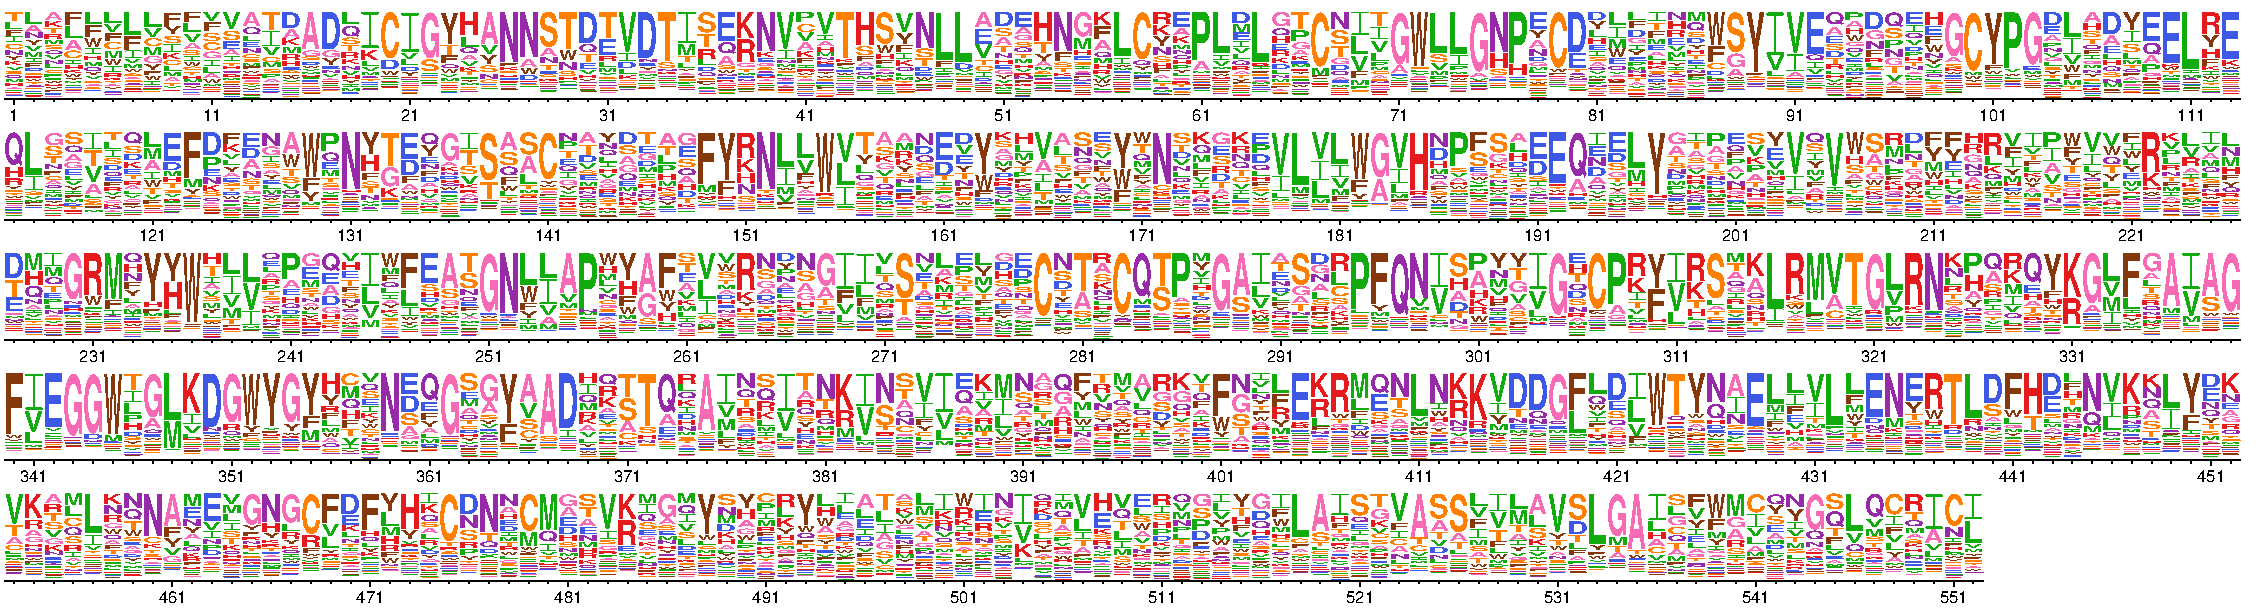
\includegraphics[width=\textwidth]{figures/prefs_doud}}
\caption{\label{suppfig:prefs_doud}
\textbf{H1 preferences measured by \cite{doud2016accurate} rescaled with the ExpCM stringency parameter optimized in \ref{fig:tree_doud}A  ($\beta = 1.19$)} 
\skhcomment{I need to change the $\beta$ value when the new \texttt{phydms} results finish running.}
}
\end{suppfig}

\begin{suppfig}[H]
\centerline{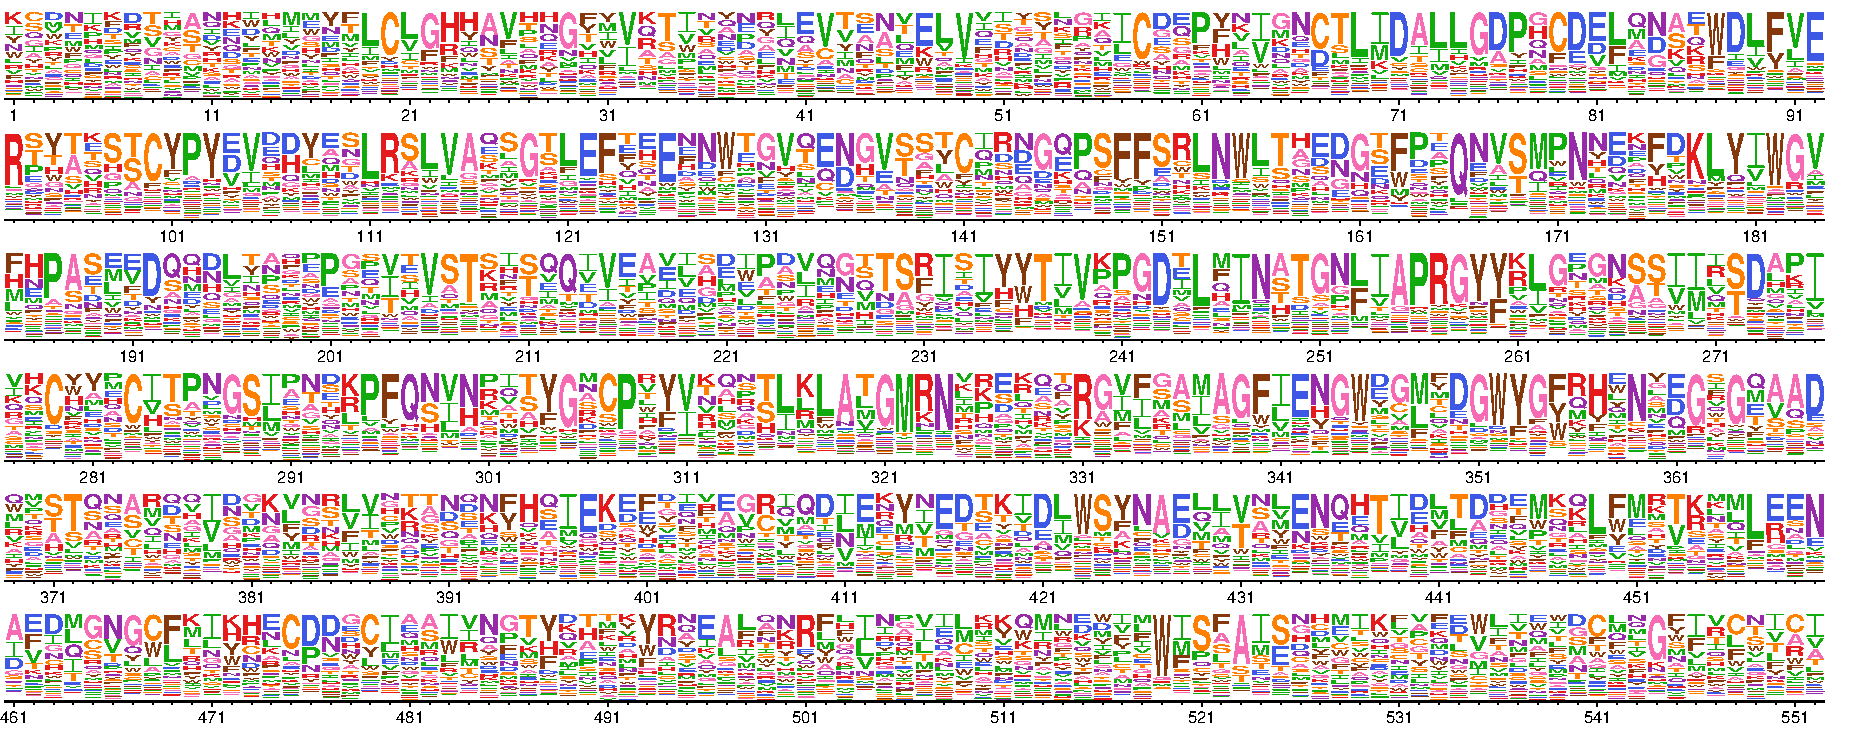
\includegraphics[width=\textwidth]{figures/prefs_lee}}
\caption{\label{suppfig:prefs_lee}
\textbf{H3 preferences measured by \textit{lee} rescaled with the ExpCM stringency parameter optimized in \ref{fig:tree_lee}A  ($\beta = 1.46$)}
\skhcomment{I need to change the $\beta$ value when the new \texttt{phydms} results finish running.} 
}
\end{suppfig}

\begin{figure}[H]
\centerline{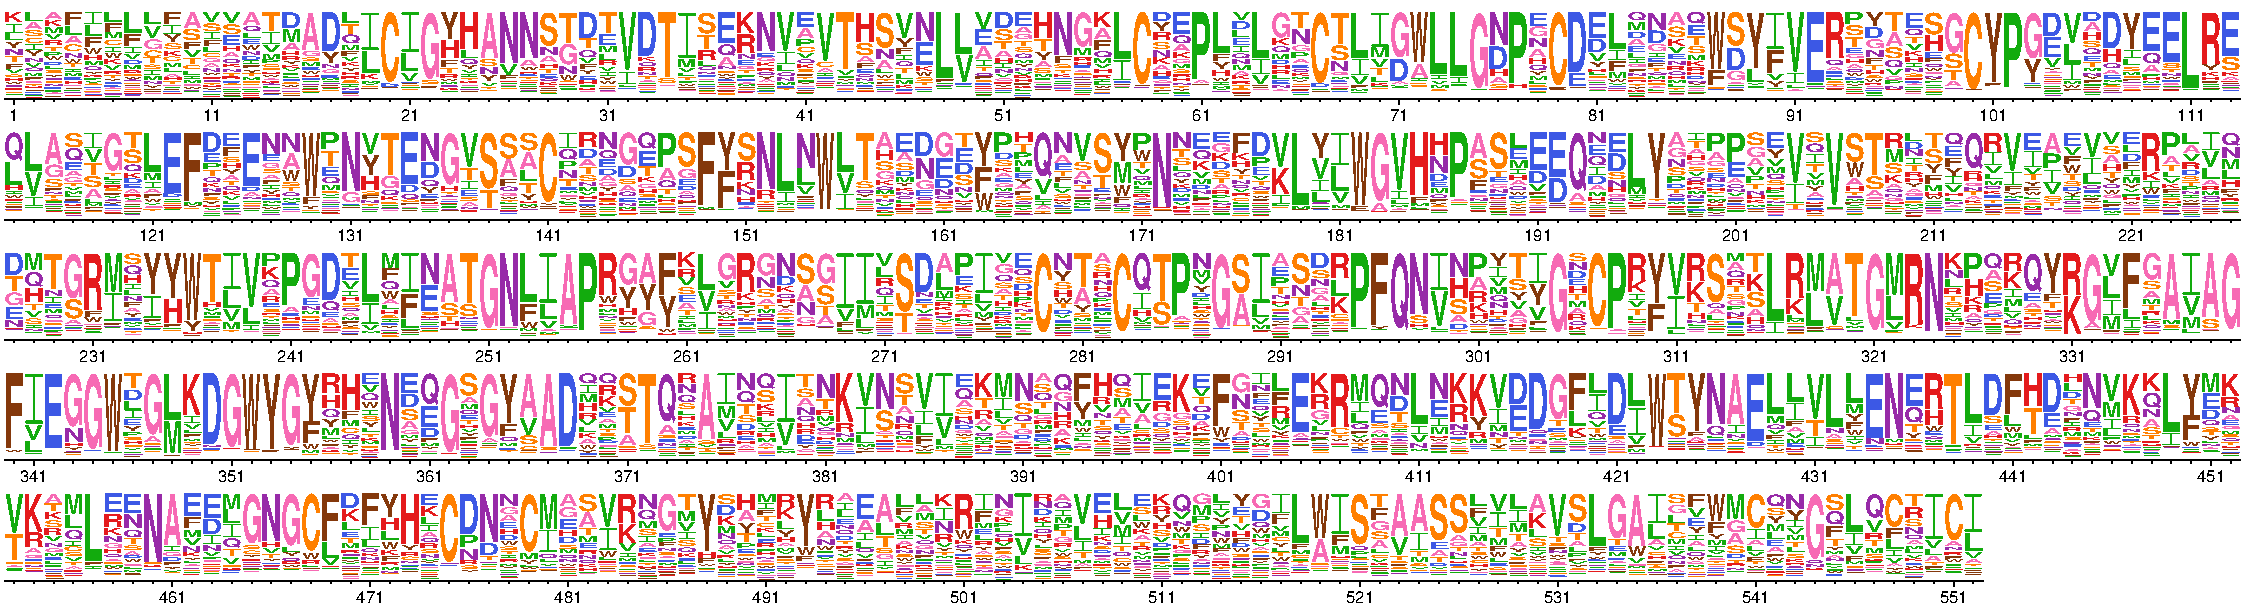
\includegraphics[width=\textwidth]{figures/prefs_average}}
\caption{\label{fig:prefs_average}
\textbf{The average of the H1 preferences measured by \cite{doud2016accurate} and the H3 preferences measured by \textit{Lee} rescaled with the ExpCM stringency parameter optimized in \ref{fig:tree_average}A  ($\beta = 1.77$)}}
\skhcomment{I need to change the $\beta$ value when the new \texttt{phydms} results finish running.}
\end{figure}



\begin{table}[t!]
\caption{\label{tab:simulation_params}
ExpCM parameters used to simulate sequences in Fig.~\ref{fig:simulation}.}
      \begin{tabular}{ccccc}
        \hline
          Parameter & Value\\ \hline
       	$\beta$ & $1.54$\\
	$\kappa$ & $3.60$\\
	$\omega$ & $0.20$\\
	$\phi_A$, $\phi_C$, $\phi_G$& $0.38$, $0.17$, $0.23$\\
      \end{tabular}
\end{table}

\begin{table}[t!]
\caption{\label{tab:wsn_low_params}
Model parameters used in  Fig.~\ref{fig:decay}.}
      \begin{tabular}{ccccc}
        \hline
          Model & Parameters\\ \hline
          ExpCM & $\beta=1.54196$\\
           & $\kappa=3.47184$\\
           & $\omega=0.219225$\\ 
          YNGKP M0 & $\kappa=2.9984$\\
          & $\omega=0.09076$\\
          YNGKP M5 & $\kappa=2.9984$\\
          & $\omega=0.09076$\\
      \end{tabular}
\end{table}

\begin{suppfig}[H]
\centerline{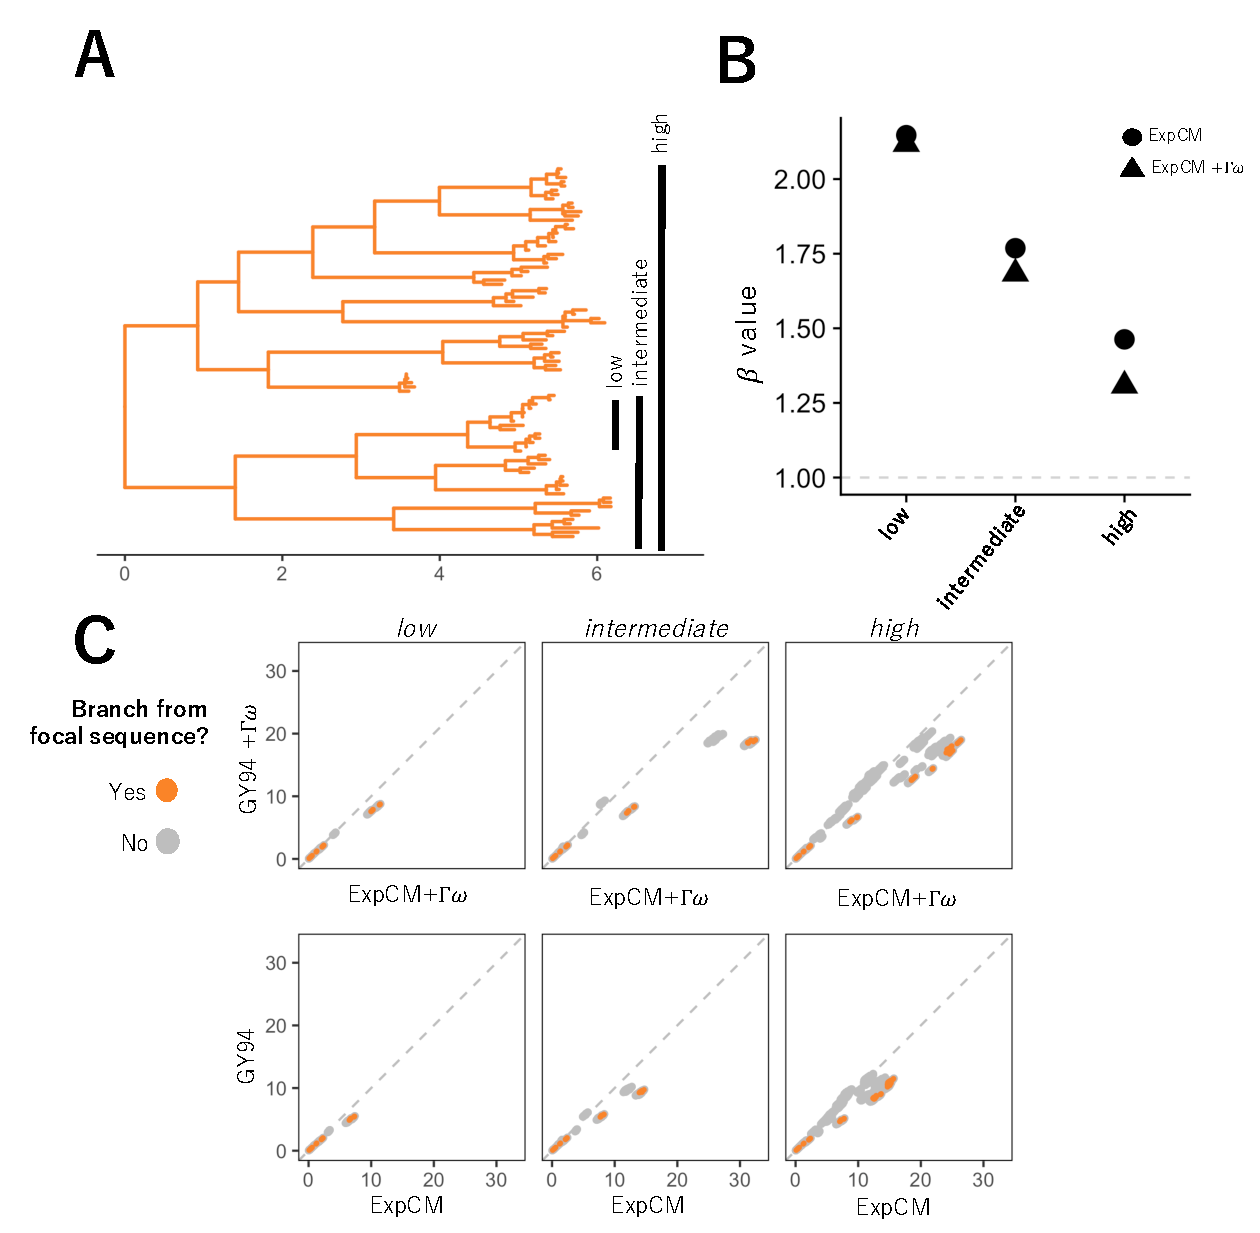
\includegraphics[width=0.85\textwidth]{figures/lee_compete}}
\caption{\label{fig:lee_compete}
\textbf{The ExpCM defined by H1 preferences lengthen longer branches on the HA tree.} 
\textbf{(A)} An HA alignment was subsampled to create three smaller alignments with varying degrees of divergence from the focal H3 sequence, referred to as "low", "intermediate", and "high". 
\textbf{(B)} The phylogenetic tree of the "high" alignment. 
The colors denote the alignment and the black circle denotes the focal H3 sequence. 
\textbf{(C)} The value of the ExpCM and ExpCM+$\Gamma\omega$ stringency parameter $\beta$ decreases as the divergence from the focal H3 sequence increases. 
\textbf{(D)} Comparisons of branch lengths optimized by the four substitution models for the varying degrees of divergence. 
Black points represent branches from the focal H3 sequence and grey points represent all other branches.  
The branch lengths are in average number of codon substitutions per site. 
}
\end{suppfig}


\clearpage 
\bibliographystyle{mbe}
\bibliography{references.bib}



\end{document}